% vim: set ts=2 sw=2 noet:
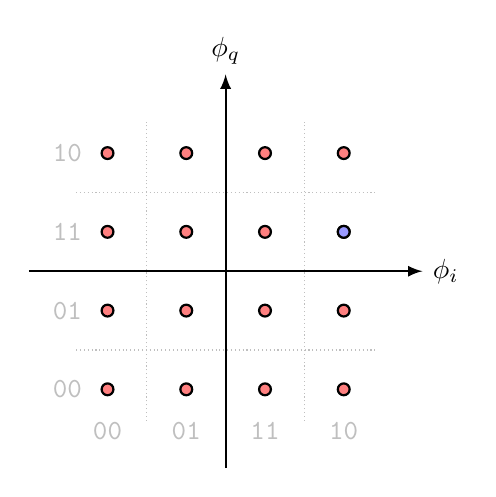
\begin{tikzpicture}[
		axis/.style = {
			thick, -latex, black,
		},
		star/.style = {
			draw = black, thick, fill = red!50,
			circle, outer sep = 1mm, inner sep = 0,
			minimum size = 1.5mm,
		},
	]

	\draw[lightgray, densely dotted, step = 10mm] (-19mm,-19mm) grid (19mm,19mm);

	\draw[axis] (-25mm,0) to (25mm,0) node[right] {\(\phi_i\)};
	\draw[axis] (0,-25mm) to (0,25mm) node[above] {\(\phi_q\)};

	\foreach \i in {0,1,...,3}{
		\foreach \q in {0,1,...,3}{
			\node[star] (s\i\q) at ({\i*10mm - 15mm},{\q*10mm - 15mm}) {};
		}
	}

	% special node for the example
	\node[star, fill = blue!40!white] at (s32) {};

	\foreach \i/\l in {0/00,1/01,2/11,3/10}{
		\node[lightgray, below = 3mm] at (s\i0) {\texttt{\l}};
		\node[lightgray, left = 2mm] at (s0\i) {\texttt{\l}};
	}
\end{tikzpicture}
